\documentclass{assignment}
\ProjectInfos*{Guided Wave Optics}{EE140}{Fall, 2020}{Assignment 3}{Due time : Dec 11, 2020 (Friday)}{陈稼霖}{45875852}
\begin{document}
\begin{prob}
    Consider the following four layer structure: $n_1=1.73$, $n_3=1.45$, $n_4=1.33$, $\lambda=0.6328\,\mu\mathrm{m}$, $d=0,10,30,50\,\mathrm{nm}$. Plot $R$ vs $\theta$ with different $d$ and $T$ vs $\theta$ with different d. You can use the software you learned in class or any software you like.
    \begin{figure}[h]
        \centering
        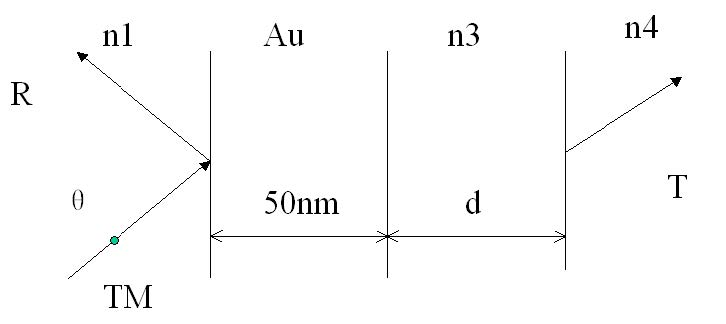
\includegraphics[width=.5\columnwidth]{A-3.jpg}
    \end{figure}
\end{prob}
\begin{sol}
    首先,查阅教科书第4章第4.2节表4.1(P80)\cite{chen2006foundations}得知金在波长$\lambda=0.6328\,\mu\mathrm{m}$处折射率约为$n_{\text{Au}}=0.17+3.0j$. 然后,编写 Lumerical 脚本,依次输入题设给定的波长、各层介质折射率和厚度,取入射角范围为$\theta\in[0,90^{\circ}]$,用 Lumerical 脚本语言内置的 stackrt 函数(算法根据传输矩阵法设计)计算在不同入射角条件下该四层介质结构对平面波的反射率和透射率,以上过程用 for 循环遍历题设给定的第三层介质厚度$d$重复进行,代码如下,各行代码对应操作见其注释.
    \begin{lstlisting}
clc; closeall; clear;
n = [1.73; 0.17 + 3.0 * 1i; 1.45; 1.33]; # 从左至右各层介质折射率
f = c / 632.8e-9; # 入射光频率(单位:Hz)
theta = 0:.1:90; # 遍历入射角(单位:度)
for(d3 = [0, 10e-9, 30e-9, 50e-9]){ # 遍历第3层介质厚度
    d = [0; 50e-9; d3; 0]; # 从左至右各层介质厚度(单位:m),其中 0 代表延伸至无穷远
    RT = stackrt(n, d, f, theta); # 用传输矩阵法计算反射率与折射率
    visualize(RT);
    plot(theta, RT.Rp, RT.Tp); # 绘制TM模反射率与折射率关于入射角变化的曲线
    setplot('y min', -.1);
    setplot('y max', 1.2);
    setplot('x label', 'Incident angle: theta / degree');
    setplot('y label', 'Reflectivity or Transmittance');
    legend('TM wave Reflectivity R','TM wave Transmittance T');
}
\end{lstlisting}
    最后,绘制在第三层介质厚度$d$取不同值的条件下,入射该四层结构的TM模平面波的反射率和透射率随入射角$\theta$变化的关系,如组图\ref{RT-theta}.
    \begin{figure}[H]
        \centering
        \subfigure[第三层介质厚度$d=0$.]{
            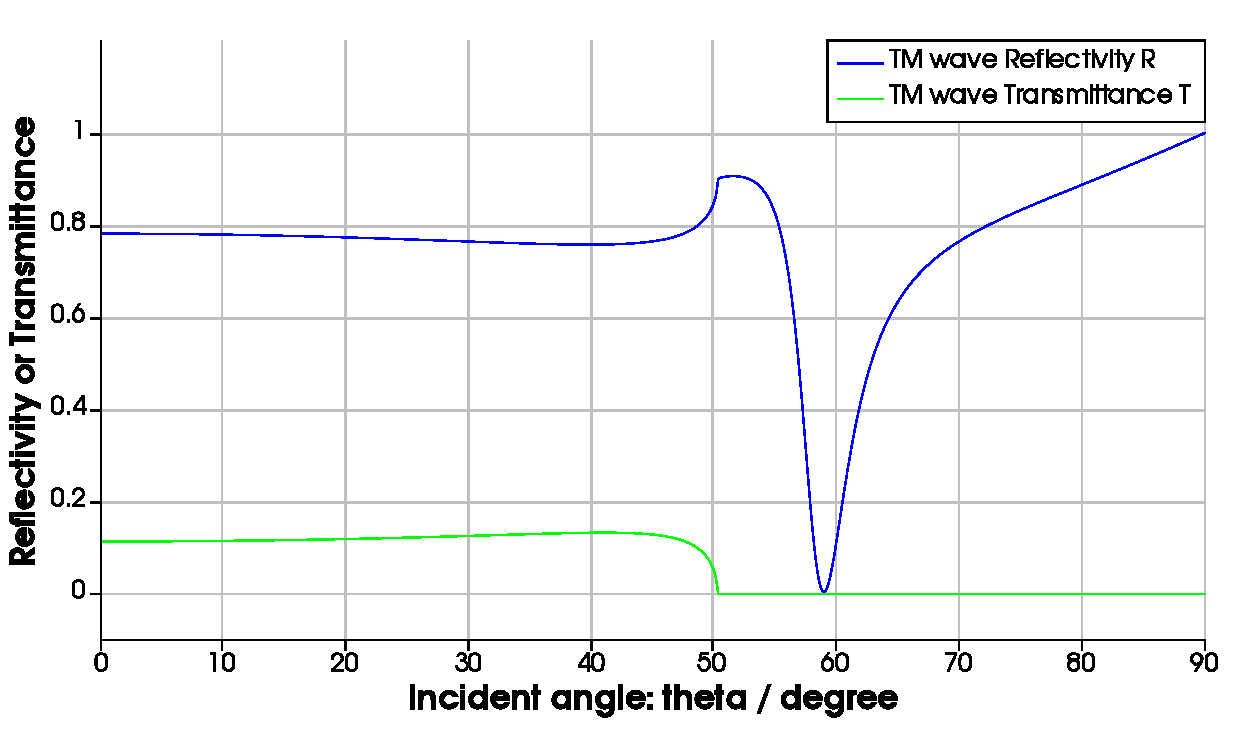
\includegraphics[width=.45\columnwidth]{RT-theta-1.pdf}
        }
        \subfigure[第三层介质厚度$d=10\,\mathrm{nm}$.]{
            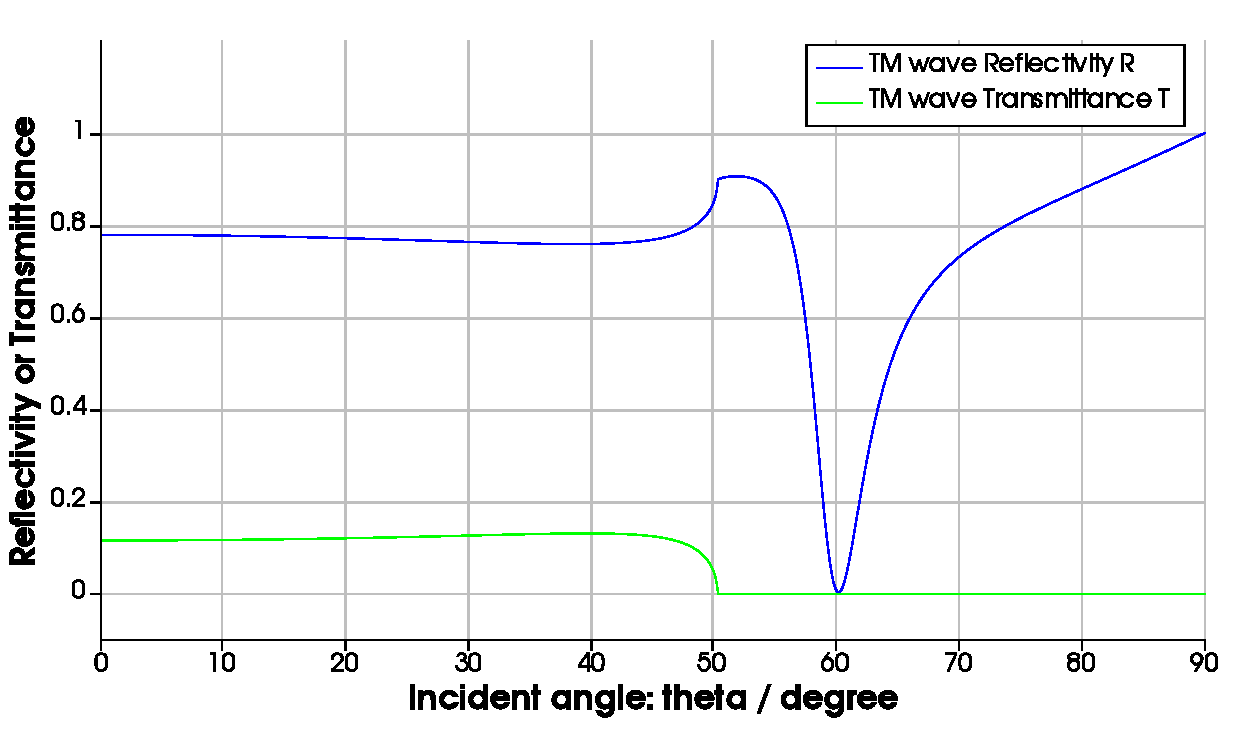
\includegraphics[width=.45\columnwidth]{RT-theta-2.pdf}
        }
        \subfigure[第三层介质厚度$d=30\,\mathrm{nm}$.]{
            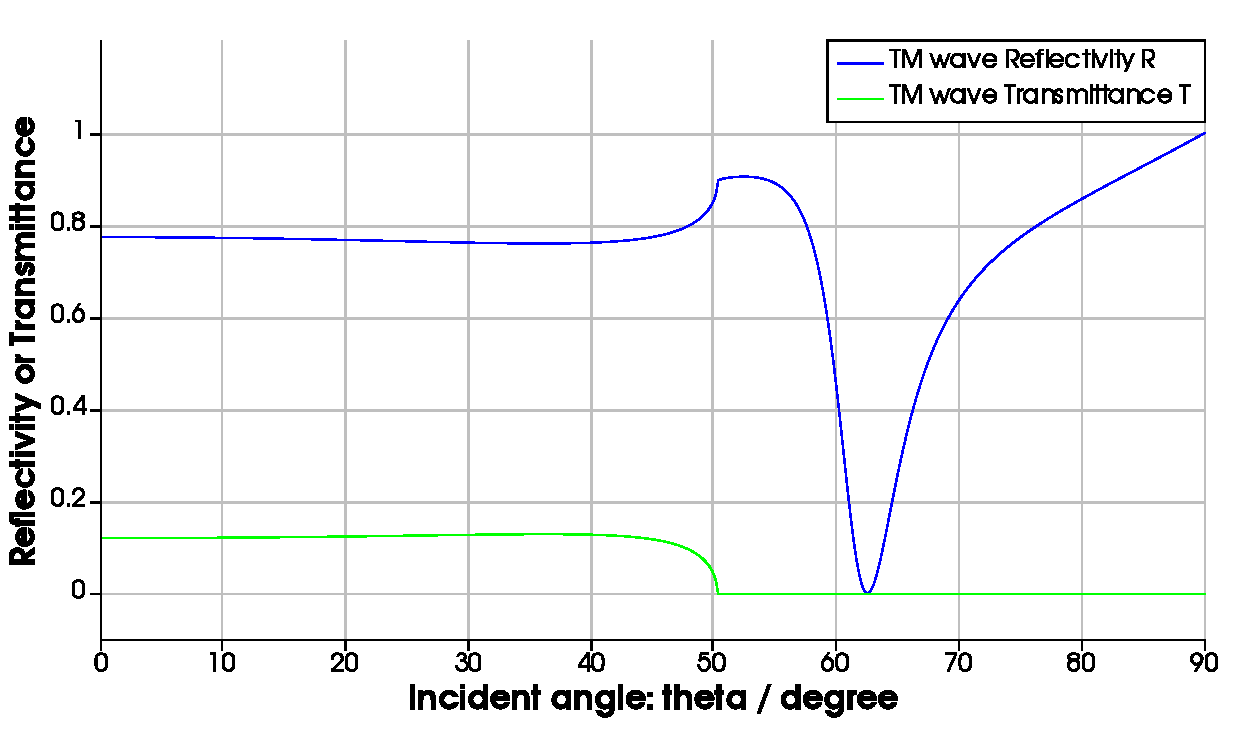
\includegraphics[width=.45\columnwidth]{RT-theta-3.pdf}
        }
        \subfigure[第三层介质厚度$d=50\,\mathrm{nm}$.]{
            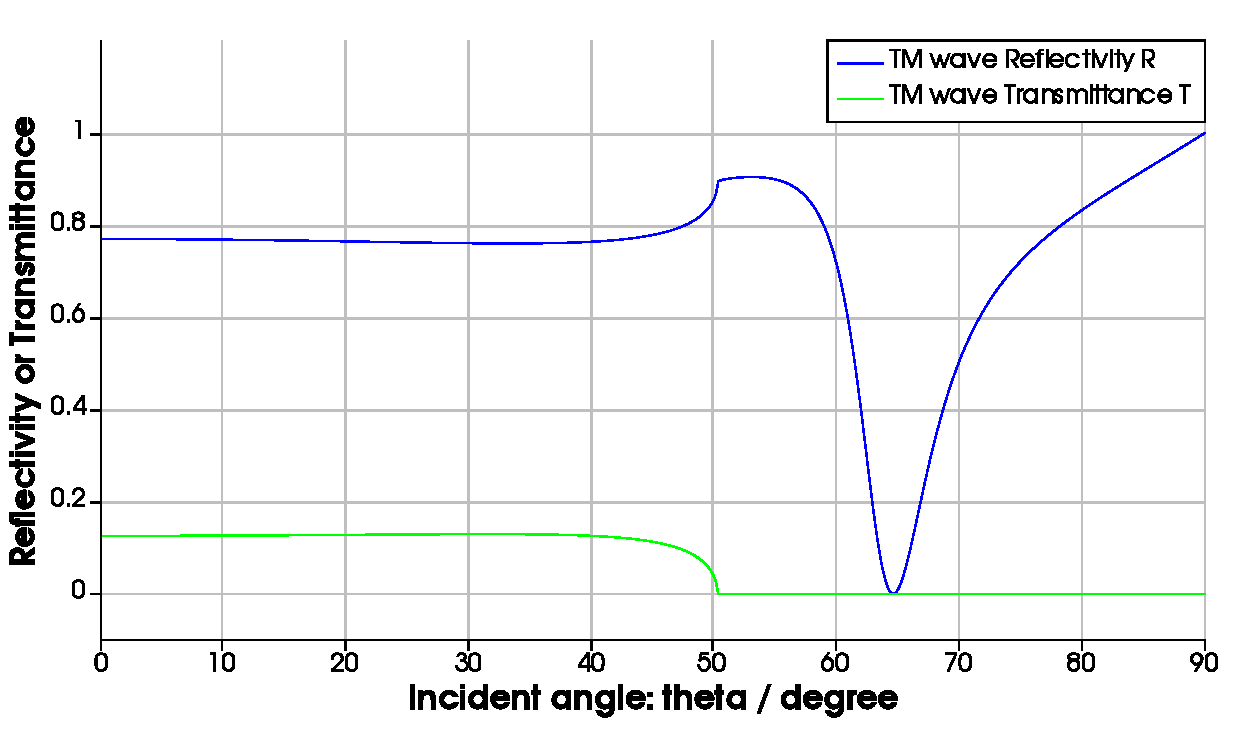
\includegraphics[width=.45\columnwidth]{RT-theta-4.pdf}
        }
        \caption{在第三层介质厚度$d$取不同值的条件下,入射该四层结构的TM模平面波的反射率和透射率随入射角$\theta$变化的关系.}
        \label{RT-theta}
    \end{figure}

    根据上面的反射率和透射率曲线,我们可以总结出以下现象:
    \begin{itemize}
        \item[(0)] 随着入射角$\theta$由$0^{\circ}$增大,TM模的反射率缓慢下降,透射率缓慢上升;
        \item[(1)] 但当$\theta$超过约$40^{\circ}$后,反射率显著上升,透射率显著下降;
        \item[(2)] 当$\theta$达到$50.3^{\circ}$,反射率达到一个极大值,而透射率降为零;
        \item[(3)] 此后继续增大入射角,折射率始终保持为零而不再改变,反射率先减小至一个接近于零的极小值,后又再次增大;
        \item[(4)] 最终反射率在$\theta=90^{\circ}$时达到$1$,
        \item[(5)] 随着第三层介质的厚度$d$的增加,反射率的极小值点右移.
    \end{itemize}

    从物理的角度,我们不难理解上面的曲线反映的现象:
    \begin{itemize}
        \item[(1)] 光由第三层介质进入第四层介质的过程,实际上是一个从光密介质入射光疏介质的过程,故当$\theta$超过约$40^{\circ}$后,随着$\theta$的继续增大,由第三层进入第四层介质时的反射率显著增大,从而光更难从第三层和第四层介质的交接面出射,因此在$40^{\circ}<\theta<50.3^{\circ}$的范围内,总透射率显著降低,而总反射率相应地显著升高;
        \item[(2)] 利用 Snell 定律,可以算出当$\theta=50.3^{\circ}$时,光在第三层和第四层介质的交界面上恰好达到全反射:
        \begin{align}
            n_1\sin\theta=n_3\sin\theta_{3\rightarrow 4,c}=n_4\sin 90^{\circ}\Longrightarrow\theta\approx 50.25^{\circ},
        \end{align}
        因此,此时完全没有任何光从第三层和第四层介质的交界面上出射,总透射率降至零,而总反射率相应地达到极大值;
        \item[(3)] 当继续增大$\theta$,光在第三层和第四层介质的交界面上全反射,从而使总透射率继续保持为零,而此时光在中间的金层和第三层介质中来回反射,由于金存在非零的折射率虚部,即金层对光场具有吸收作用,而$\theta$增大,光在金层中走过的路程变长,金层对光的总吸收率增大,因此总反射率相应地降低,而又因为从第一层介质到金层的反射率随着$\theta$的增大而增大,故再继续增大$\theta$,进入金层的光的比例减小,金层对光的总吸收量减小,因此总反射率再次增大;
        \item[(4)] 最终当$\theta=90^{\circ}$时,入射平面波平行于第一层介质与金层间的交界面传播,完全不进入金层,因此反射率达到$1$,
        \item[(5)] 增大$d$意味着,第三层介质对光的束缚能力变强(准确地说,光在中间两层介质中传播的时间内,有更大比例的时间是被第三层介质所容纳的),因此金层对光的吸收作用相对减小了,从而延缓了反射率极小值的到来.
    \end{itemize}
\end{sol}

\bibliographystyle{plain}
\bibliography{References}
\end{document}